%%%%%%%%%%%%%%%%%%%%%%%%%%%%%%%%%%%%%%%%%
% Short Sectioned Assignment LaTeX Template Version 1.0 (5/5/12)
% This template has been downloaded from: http://www.LaTeXTemplates.com
% Original author:  Frits Wenneker (http://www.howtotex.com)
% License: CC BY-NC-SA 3.0 (http://creativecommons.org/licenses/by-nc-sa/3.0/)
%%%%%%%%%%%%%%%%%%%%%%%%%%%%%%%%%%%%%%%%%

%----------------------------------------------------------------------------------------
%   PACKAGES AND OTHER DOCUMENT CONFIGURATIONS
%----------------------------------------------------------------------------------------

\documentclass[10pt,a4paper,spanish]{article}

% ---- Entrada y salida de texto -----

\usepackage[spanish]{babel} 
\usepackage[T1]{fontenc} % Use 8-bit encoding that has 256 glyphs
\usepackage[utf8]{inputenc}
\usepackage{minted}
% \usepackage{fourier} % Use the Adobe Utopia font for the document - comment this line to return to the LaTeX default
\usepackage[usenames, dvipsnames]{color}
\usepackage{xcolor}
\usepackage{colortbl}
\usepackage[bookmarks=true,colorlinks=true,linkcolor=red,citecolor=blue]{hyperref}
\usepackage{cite}
\usepackage[official]{eurosym}
\usepackage{tikz}
\usepackage{pgfplots}
\pgfplotsset{compat=1.5}
% \usepackage{pgf-pie}
\usepackage{subfigure}

% ---- Otros paquetes ----
\usepackage{enumerate}
\usepackage{amsmath,amsfonts,amsthm,amssymb} % Math packages
\usepackage{graphics,graphicx} %para incluir imágenes y notas en las imágenes
% Para hacer tablas comlejas
%\usepackage{multirow}
%\usepackage{threeparttable}

\usepackage[a4paper, margin=1.3in]{geometry}


\usepackage{sectsty} % Allows customizing section commands
\allsectionsfont{\centering \normalfont\bfseries\scshape} % Make all sections centered, the default font and small caps

\usepackage{fancyhdr} % Custom headers and footers
\pagestyle{fancyplain} % Makes all pages in the document conform to the custom headers and footers
\fancyhead{} % No page header - if you want one, create it in the same way as the footers below
\fancyfoot[L]{} % Empty left footer
\fancyfoot[C]{} % Empty center footer
\fancyfoot[R]{\thepage} % Page numbering for right footer
\renewcommand{\headrulewidth}{0pt} % Remove header underlines
\renewcommand{\footrulewidth}{0pt} % Remove footer underlines
\setlength{\headheight}{13.6pt} % Customize the height of the header

\numberwithin{equation}{section} % Number equations within sections (i.e. 1.1, 1.2, 2.1, 2.2 instead of 1, 2, 3, 4)
\numberwithin{figure}{section} % Number figures within sections (i.e. 1.1, 1.2, 2.1, 2.2 instead of 1, 2, 3, 4)
\numberwithin{table}{section} % Number tables within sections (i.e. 1.1, 1.2, 2.1, 2.2 instead of 1, 2, 3, 4)

\setlength\parindent{0pt} % Removes all indentation from paragraphs - comment this line for an assignment with lots of text
\setlength{\parskip}{1ex plus 0.5ex minus 0.2ex}

\newcommand{\horrule}[1]{\rule{\linewidth}{#1}} % Create horizontal rule command with 1 argument of height

%----------------------------------------------------------------------------------------
%   TÍTULO Y DATOS DEL ALUMNO
%----------------------------------------------------------------------------------------

\title{
\normalfont \normalsize 
\textsc{{\bf Ingeniería de Servidores (2015-2016)} \\ Grado en Ingeniería Informática \\ Universidad de Granada} \\ [25pt] % Your university, school and/or department name(s)
\horrule{0.5pt} \\[0.4cm] % Thin top horizontal rule
\huge Memoria Práctica 2 \\ % The assignment title
\horrule{2pt} \\[0.5cm] % Thick bottom horizontal rule
}

\author{Marta Gómez Macías} % Nombre y apellidos

\date{\normalsize\today} % Incluye la fecha actual

\newmintedfile[mybash]{bash}{
    linenos,
    numbersep=5pt,
    gobble=0,
    frame=lines,
    framesep=2mm,
    tabsize=3,
}

\newmintedfile[myyml]{yaml}{
    linenos,
    numbersep=5pt,
    gobble=0,
    frame=lines,
    framesep=2mm,
    tabsize=3,
}

\newmintedfile[mycpp]{cpp}{
    linenos,
    numbersep=5pt,
    gobble=0,
    frame=lines,
    framesep=2mm,
    tabsize=3,
}

\newmintedfile[mydiff]{diff}{
    linenos,
    numbersep=5pt,
    gobble=0,
    frame=lines,
    framesep=2mm,
    tabsize=3,
}


%----------------------------------------------------------------------------------------
% DOCUMENTO
%----------------------------------------------------------------------------------------

\begin{document}
%Cambiar Cuadros por Tablas y lista de...
\renewcommand{\listtablename}{Índice de tablas}
\renewcommand{\tablename}{Tabla} 

\maketitle % Muestra el Título
\pagenumbering{gobble} 

\newpage %inserta un salto de página
\pagenumbering{arabic} 

\tableofcontents % para generar el índice de contenidos

\listoffigures

% \listoftables

\newpage

\section{Liste los argumentos de \texttt{yum} necesarios para instalar, buscar y eliminar paquetes}
Si miramos en \cite{manyum}, nos vienen los comandos que podemos utilizar según lo que queramos hacer. En concreto los comandos que se piden en el enunciado son:
\begin{enumerate}[---]
    \item \texttt{yum install}:
    \begin{minted}{bash}
    yum install package1 [package2] [...]
    \end{minted}

    Se usa para instalar la última versión de un paquete o grupo de paquetes asegurándose de que se cumplen todas las dependencias. Tiene varias peculiaridades:
    \begin{enumerate}[$\bullet$]
        \item Si empieza por el carácter $@$ busca grupos de paquetes.
        \item Si el nombre es un archivo, instala un paquete local, como si llamásemos al comando \texttt{yum localinstall}
    \end{enumerate}

    \item \texttt{yum erase} o \texttt{yum remove}:
    \begin{minted}{bash}
    yum remove package1 [package2] [...]
    \end{minted}

    Se usa para borrar los paquetes que especifiquemos y sus dependencias. La operación sobre los grupos de archivos funciona igual que en el comando \texttt{install}.

    \item \texttt{yum search}
    \begin{minted}{bash}
    yum search string1 [string2] [...]
    \end{minted}

    Se usa para buscar paquetes cuando no estamos seguros de cómo se llaman. Por defecto busca nombres de paquetes y sumarios, pero también podemos buscar por descripción y URL.
\end{enumerate}

\section{¿Qué ha de hacer para que yum pueda tener acceso a internet¿ ¿Cómo añadimos un nuevo repositorio?}
Tal y como se especifica en \cite{proxycentos}, debemos modificar el archivo \textit{/etc/yum.conf} y añadir la siguiente línea:

\begin{minted}[frame=single, label={Configuración del proxy en yum}]{bash}
# The proxy server - proxy server:port number
proxy=stargate.ugr.es:312
\end{minted}

Para añadir un nuevo repositorio, según \cite{addrepo}, debemos ejecutar el siguiente comando:

\begin{minted}[frame={single}, label={Añadir un nuevo repositorio en yum}]{bash}
yum-config-manager --add-repo repository_url
\end{minted}

Donde \texttt{repository\_url} es un enlace al archivo \textbf{.repo}. 

Una vez hecho esto, para activar el respositorio debemos ejecutar el siguiente comando:
\begin{minted}[frame={single}, label={Activar un repositorio en yum}]{bash}
yum-config-manager --enable repository
\end{minted}

Donde \texttt{respository} es el ID del repositorio (si no lo sabemos, usamos \texttt{yum repolist all} para listar los IDs disponibles). También podemos usar expresiones globales para activar todos los respositorios que coincidan con dicha expresión global.

Este comando tiene la misma sintaxis que el que se usa para desactivar un repositorio:
\begin{minted}[frame={single}, label={Desactivar un repositorio en yum}]{bash}
yum-config-manager --disable repository
\end{minted}

\section{Indique el comando para buscar un paquete en un repositorio y el correspondiente para instalarlo}
En \cite{manapt}, nos citan las distintas páginas de manual que tienen que ver con \texttt{apt}. En concreto, las que nos interesan son:

\begin{enumerate}[---]
    \item \texttt{apt-chache}: según \cite{manaptchache}, usando el comando \texttt{search} busca en todas las listas de repositorios disponibles para el patrón dado. Éste puede contener expresiones regulares. Por defecto nos muestra el nombre del paquete y una pequeña descripción, pero podemos modificar este comportamiento:
    \begin{enumerate}[$\bullet$]
        \item \texttt{--full}: muestra una descripción completa del paquete, el output es el mismo que con el comando \texttt{show}.
        \item \texttt{--names-only}: sólo busca paquetes por su nombre.
    \end{enumerate}

    \item \texttt{apt-get}: según \cite{manaptget}, usando el comando \texttt{install} seguido del nombre de uno o más paquetes, instalará los paquetes dados. Si el nombre del paquete lleva delante el símbolo $-$ eliminará el paquete si está instalado, y si lleva el signo $+$, lo instalará. También podemos seleccionar una versión concreta de un paquete con el símbolo $=$ seguido de la versión deseada. Por último, podemos usar expresiones regulares para instalar o eliminar todos los paquetes que coincidan.
\end{enumerate}

\section{Indique qué ha modificado para que \texttt{apt} pueda acceder a los servidores de paquetes a través del proxy. ¿Cómo añadimos un nuevo repositorio?}
Tal y como se explica en \cite{aptproxy}, para acceder a un proxy por HTTP debemos añadir la siguiente línea o bien al archivo \textit{/etc/apt/apt.conf} (\cite{manaptconf}) o bien al \textit{/etc/apt/apt.conf.d/proxy}:

\begin{minted}[frame=single, label={Configurar un servidor proxy}]{bash}
Acquire::http::Proxy "http://stargate.ugr.es:312";
\end{minted}

Si no existen los archivos, creamos uno de ellos.

En \cite{addrepoubu}, nos explican el comando \texttt{add-apt-repository}, con el cual podemos añadir un repositorio a apt. En la \hyperref[addrepository]{Figura \ref*{addrepository}} vemos el output al ejecutar el comando con la opción \texttt{-h}. Así, podemos saber las distintas opciones con las que podemos ejecutarlo.

\begin{figure}[!h]
\centering
\mbox {
\subfigure[Primera parte del output de \texttt{add-apt-repository -h}]{
\label{uno}
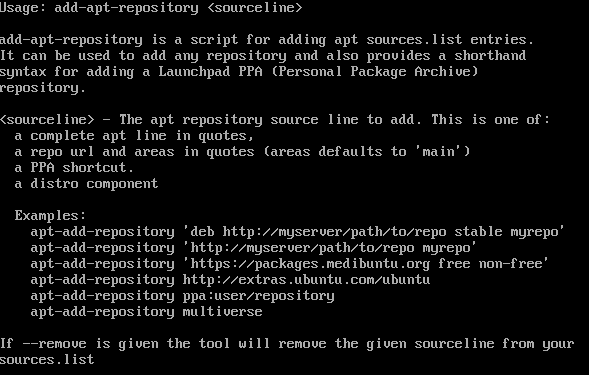
\includegraphics[width=0.5\textwidth]{1}
}
\qquad
\subfigure[Segunda parte del output de \texttt{add-apt-repository -h}] {
\label{dos}
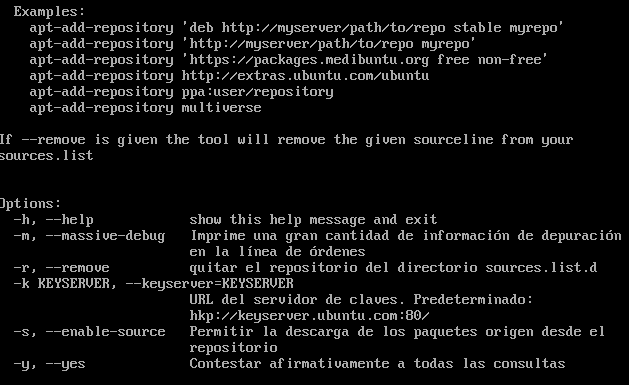
\includegraphics[width=0.5\textwidth]{2}
}
}
\caption{Output de \texttt{add-apt-repository -h}}
\label{addrepository}
\end{figure}

\section{¿Qué diferencua hay entre telnet y shh?}
Tal y como se explica en el primer párrafo de \cite{openssh}, telnet envía las contraseñas sin encriptar mientras que SSH sí. Pero no sólo las contraseñas sino todo el tráfico. 

\section{¿Para qué sirve la opción \texttt{-X}? Ejecute remotamente, es decir, desde la máquina anfitriona o desde la otra máquina virtual, el comando \texttt{gedit} en una sesión abierta con \texttt{ssh}. ¿Qué ocurre?}

Consultando \cite{manssh} podemos ver las distintas opciones que acepta con una explicación, en concreto, la opción \texttt{-X} nos dice que sirve para activar el \textit{X11 forwading}\footnote{Según \cite{x11}, el X11 forwading es el sistema de ventanas X que nos permite ejecutar aplicaciones en un servidor UNIX como si estuviésemos ejecutando aplicaciones en Windows pudiendo incluso usar el ratón en éstas.}

Al ejecutar \texttt{gedit} en una sesión \texttt{ssh} desde la máquina remota, se nos abre una ventana de gedit normal, pero que se está ejecutando en la máquina anfitriona. Tal y como se ve en la \hyperref[sshgedit]{Figura \ref*{sshgedit}}, tenemos una ventana de gedit ejecutándose, pero al hacer \texttt{ps} en la máquina local no encuentra ningún proceso \texttt{gedit} activo. En cambio, al hacer \texttt{ps} en la sesión remota, sí.

\begin{figure}[!h]
\centering
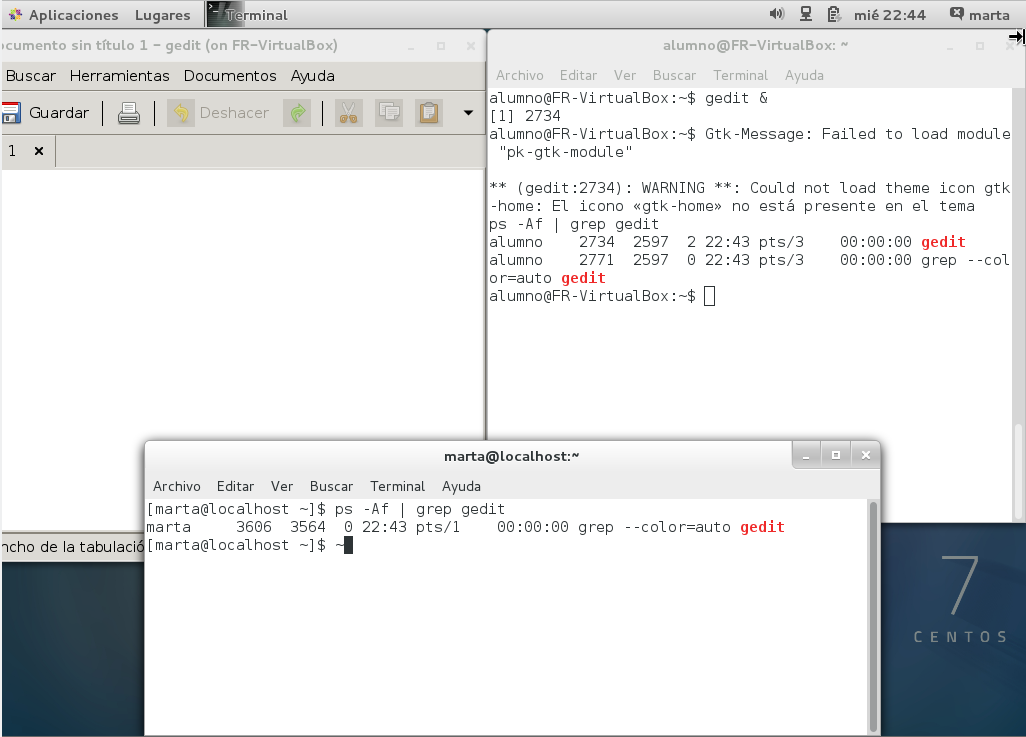
\includegraphics[width=0.75\textwidth]{3}
\caption{Ejecutando \texttt{gedit} desde una sesión \texttt{ssh}}
\label{sshgedit}
\end{figure}

\section{Muestre la secuencia de comandos y las modificaciones a los archivos correspondientes para permitir acceder a la consola remota sin introducir la contraseña.}

Para crear la clave pública y privada en el cliente, se han seguido los pasos indicados en \cite{gitssh}. Para transferir la clave pública creada al servidor, se han seguido los pasos indicados en \cite{ubussh}.

\subsection{Creando la clave pública y privada en el cliente}
En primer lugar, comprobamos que no tenemos ninguna clave generada en nuestro ordenador, para ello listamos el contenido del directorio de ssh:

\begin{minted}[frame=single, label={Lista los archivos del directorio .ssh}]{bash}
ls -al ~/.ssh
\end{minted}

En nuestro caso, como se aprecia en la \hyperref[lsssh]{Figura \ref*{lsssh}} no tenemos ninguna clave generada.

\begin{figure}[!h]
    \centering
    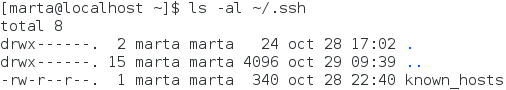
\includegraphics[width=0.75\textwidth]{4}
    \caption{Comprobando que no tenemos ninguna clave generada anteriormente}
    \label{lsssh}
\end{figure}

Como no tenemos ninguna clave, pasamos a generarla usando nuestro nombre como etiqueta:

\begin{minted}[frame=single, label={Crea una nueva clave ssh}]{bash}
ssh-keygen -t rsa -b 4096 -C "marta"
\end{minted}

tras esto, nos pedirá que elijamos un archivo en el que guradar la clave, se recomienda dejarlo por defecto pulsando enter. Por último, nos pide introducir una clave, si pulsamos enter no pondrá ninguna clave al archivo pero lo recomendable es ponerle una.

Así, finalmente nos dará nuestro \textit{fingerprint} de nuestra clave SSH. El output de este comando es el que se ve en la \hyperref[clavessh]{Figura \ref*{clavessh}}.

\begin{figure}[!h]
    \centering
    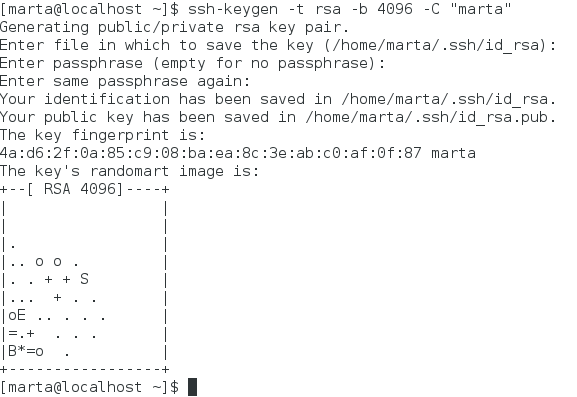
\includegraphics[width=0.75\textwidth]{5}
    \caption{Output tras generar nuestra clave}
    \label{clavessh}
\end{figure}

Por último, añadimos nuestra clave ssh al agente de ssh. Para ello, en primer lugar nos aseguramos de que está activado:

\begin{minted}[frame=single, label={Arrancamos el agente ssh}]{bash}
eval "$(ssh-agent -s)"
\end{minted}

Aunque en mi caso el comando \texttt{eval} no funcionó y tuve que hacer sólo \texttt{ssh-agent -s}, tal y como se ve en la \hyperref[sshagent]{Figura \ref*{sshagent}}.

\begin{figure}[!h]
\centering
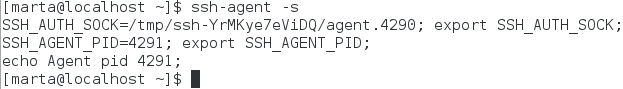
\includegraphics[width=0.75\textwidth]{6}
\caption{Arrancando el agente ssh}
\label{sshagent}
\end{figure}

Por último, añadimos la clave al agente ssh:

\begin{minted}[frame=single, label={Añade la clave generada al agente}]{bash}
ssh-add ~/.ssh/id_rsa
\end{minted}

Tras hacer esto nos da un mensaje de que todo ha ido bien, tal y como se ve en la \hyperref[claveadd]{Figura \ref*{claveadd}}.

\begin{figure}[!h]
    \centering
    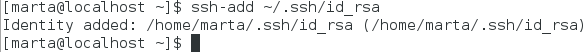
\includegraphics[width=0.75\textwidth]{7}
    \caption{Añadiendo la clave generada al agente ssh}
    \label{claveadd}
\end{figure}

\subsection{Transfiriendo la clave pública creada al servidor}
En la máquina desde la que queremos acceder, usamos el siguiente comando para transferir la clave:

\begin{minted}[frame=single, label={Copiando la clave pública al servidor}]{bash}
ssh-copy-id <username>@<host>
\end{minted}

Donde \texttt{<username>} y \texttt{<host>} deben ser reemplazados por el nombre de usuario correspondiente y la IP de la máquina a la que le estás transfiriendo tu clave.

Tras esto nos pedirá la contraseña del usuario y por último nos mostrará un mensaje de éxito tal y como se ve en la \hyperref[copyid]{Figura \ref*{copyid}}.

\begin{figure}[!h]
    \centering
    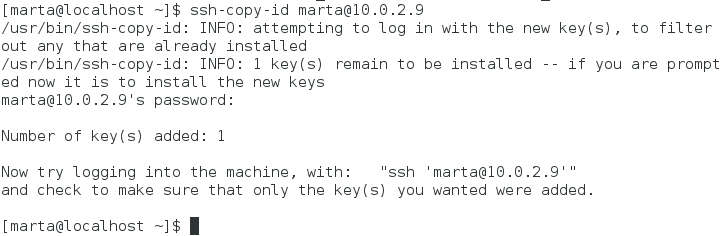
\includegraphics[width=0.75\textwidth]{8}
    \caption{Copiando la clave pública al servidor}
    \label{copyid}
\end{figure}

Por último, comprobamos que hemos copiado bien la clave accediendo por ssh y comprobando que no nos pide contraseña, tal y como se ve en la \hyperref[fin]{Figura \ref*{fin}}.

\begin{figure}[!h]
    \centering
    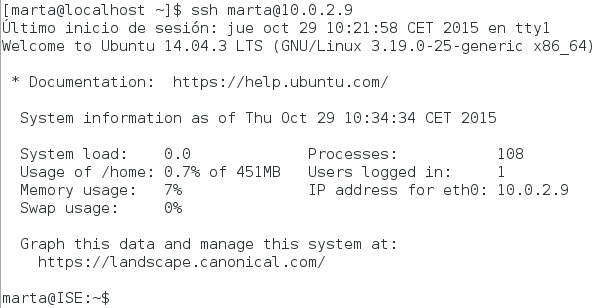
\includegraphics[width=0.75\textwidth]{9}
    \caption{Comprobando que todo ha ido bien}
    \label{fin}
\end{figure}

\section{¿Qué archivo es el que contiene la configuración de sshd? ¿Qué parámetro hay que modificar para evitar que el usuario root acceda? Cambie el puerto por defecto y compruebe que puede acceder}
Según \cite{mansshd}, el archivo de configuración del demonio de ssh es \textit{/etc/ssh/sshd\_config}. Para que el root no pueda acceder, debemos modificar el parámetro \textbf{PermitRootLogin}. Este parámetro puede tomar varios valores:
\begin{enumerate}[$\heartsuit$]
    \item \textbf{yes}: el valor por defecto.
    \item \textbf{without-password}: se desactiva la autentificación por contraseña del root.
    \item \textbf{forced-commands-only}: se permitirá el login con clave pública pero sólo si la opción \textit{command} se especifica. Cualquier otro método de autentificación queda desactivado para el root.
    \item \textbf{no}: no permite que root se loguee.
\end{enumerate}

en nuestro caso, debemos modificarlo por el valor \textbf{no}.

Para cambiar el puerto por defecto, en el mismo archivo de configuración debemos cambiar el valor del parámetro \textbf{Port}. Tras esto, intentamos conectarnos desde la máquina cliente y la conexión se realiza con éxito (en el puerto 22).

\section{Indique si es necesario reiniciar el servicio ¿Cómo se reinicia un servicio en Ubuntu? ¿y en CentOS? Muestra la secuencia de comandos para hacerlo.}
\subsection{Ubuntu}
Tal y como se indica en \cite{ubuconf}, tras hacer algún cambio en la configuración de SSH debemos reiniciar el servicio con el comando
\begin{minted}[frame=single, label={Reiniciando el servicio SSH}]{bash}
sudo restart ssh
\end{minted}

Una vez hecho esto, intentamos conectarnos de nuevo desde el cliente y nos da el error de la \hyperref[errorssh]{Figura \ref*{errorssh}}.

\begin{figure}[!h]
    \centering
    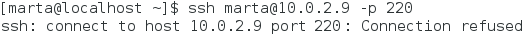
\includegraphics[width=0.75\textwidth]{13}
    \caption{Error al conectarnos al servicio SHH tras cambiar el puerto}
    \label{errorssh}
\end{figure}

Es decir, debemos abrir el nuevo puerto asignado al servicio SSH:

\begin{minted}[frame=single, label={Abriendo el puerto 220}]{bash}
sudo iptables -A INPUT -p tcp -i eth0 --dport 220 -j ACCEPT
\end{minted}

Tras esto, intentamos loguearnos y esta vez, lo hacemos con éxito tal y como se ve en la \hyperref[puerto]{Figura \ref*{puerto}}.

\begin{figure}[!h]
    \centering
    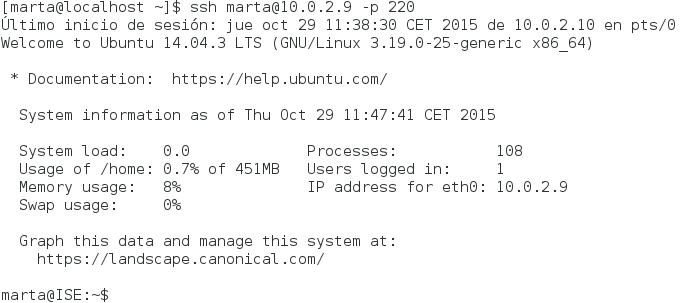
\includegraphics[width=0.75\textwidth]{14}
    \caption{Tras abrir el puerto, nos podemos loguear}
    \label{puerto}
\end{figure}

\subsection{CentOS}
Para reiniciar un servicio en CentOS, tal y como se indica en el capítulo \textit{Managing Services With Systemd} de \cite{redhatctl}, se debe usar el comando \texttt{systemctl}. En nuestro caso, para reiniciar el servicio SSH usaremos el comando:
\begin{minted}[frame=single, label={Reiniciando el servicio SSH}]{bash}
sudo systemctl restart sshd
\end{minted}

\section{Muestre los comandos que ha utilizado en Ubuntu Server y en CentOS (aunque en este último puede utilizar la GUI, en tal caso, relice capturas de pantalla) para instalar un servidor web LAMP}
\subsection{Ubuntu Server}
Siguiendo los pasos especificados en \cite{digocean} y partiendo de una instalación de Ubuntu, seguimos los siguientes pasos:

\begin{enumerate}[1.]
    \item En primer lugar instalamos el servidor Apache:
    \begin{minted}[frame=single, label={Instalando el servidor web Apache}]{bash}
    sudo apt-get install apache2
    \end{minted}

    Como estamos usando una interfaz de consola, no podemos comprobar que se ha configurado bien el servidor visitando \texttt{http://10.0.2.9}.

    \item En segundo lugar, instalamos MySQL:
    \begin{minted}[frame=single, label={Instalando MySQL}]{bash}
    sudo apt-get install mysql-server php5-mysql
    \end{minted}

    durante la instalación nos pedirá una contraseña para el administrador de la base de datos, tal y como se ve en la \hyperref[passmysql]{Figura \ref*{passmysql}}.
    \begin{figure}[!h]
        \centering
        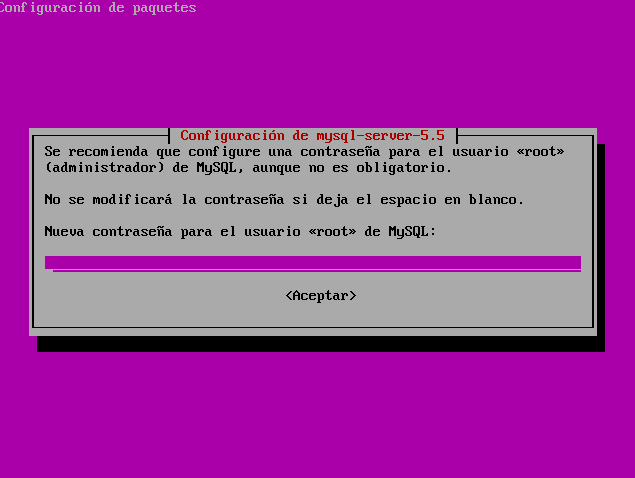
\includegraphics[width=0.5\textwidth]{15}
        \caption{Configurando la contraseña del administrador de la base de datos}
        \label{passmysql}
    \end{figure}

    \item Tras la instalación, debemos decirle al gestor de base de datos que cree su propia estructura de directorios donde guardar su información:
    \begin{minted}[frame=single, label={Creando la estructura de directorios de la base de datos}]{bash}
    sudo mysql_install_db
    \end{minted}

    También podemos hacer una instalación interactiva y personalizada para quitar algunas opciones por defecto algo peligrosas con:
    \begin{minted}[frame=single, label={Instalación manual de la base de datos}]{bash}
    sudo mysql_secure_installation
    \end{minted}

    En la cual seguiremos los siguientes pasos:
    \begin{enumerate}[1.]
        \item Nos pedirá hacer login con el root, si no tenemos contraseña nos dirá que establezcamos una.
        \item En segundo lugar nos dirá si eliminamos los usuarios anónimos de la base de datos.
        \item En tercer lugar nos dirá si desactivamos el acceso root remoto.
        \item Después, nos dirá si se elimina la base de datos por defecto \textit{test} con la que viene.
        \item Y por último, nos dirá si se recarga la tabla de privilegios.
    \end{enumerate}

    \item Tras esto, instalamos PHP:
    \begin{minted}[frame=single, label={Instalando PHP}]{bash}
    sudo apt-get install php5 libapache2-mod-php5 php5-mcrypt
    \end{minted}
\end{enumerate}

\subsection{CentOS}
Siguiendo los pasos indicados en \cite{digocean2}, los comandos para instalar un servidor LAMP han sido:
\begin{enumerate}[1.]
    \item En primer lugar instalamos Apache. Para ello, ejecutamos el siguiente comando de terminal
    \begin{minted}[frame=single, label={Instalación de Apache}]{bash}
    sudo yum install httpd
    \end{minted}

    \item Una vez instalado, empezamos a ejecutarlo:
    \begin{minted}[frame=single, label={Arranque del servidor}]{bash}
    sudo service httpd start
    \end{minted}

    \item Para comprobar que funciona, metemos en nuestro navegador \texttt{http://ip\_de\_nuestro\_servidor} y nos deberá aparecer ĺa página que se ve en la \hyperref[apacheok]{Figura \ref*{apacheok}}.
    \begin{minted}[frame=single, label={Probando si nuestro servidor ha sido instalado correctamente}]{bash}
    firefox http://10.0.2.10
    \end{minted}

    \begin{figure}[!h]
        \centering
        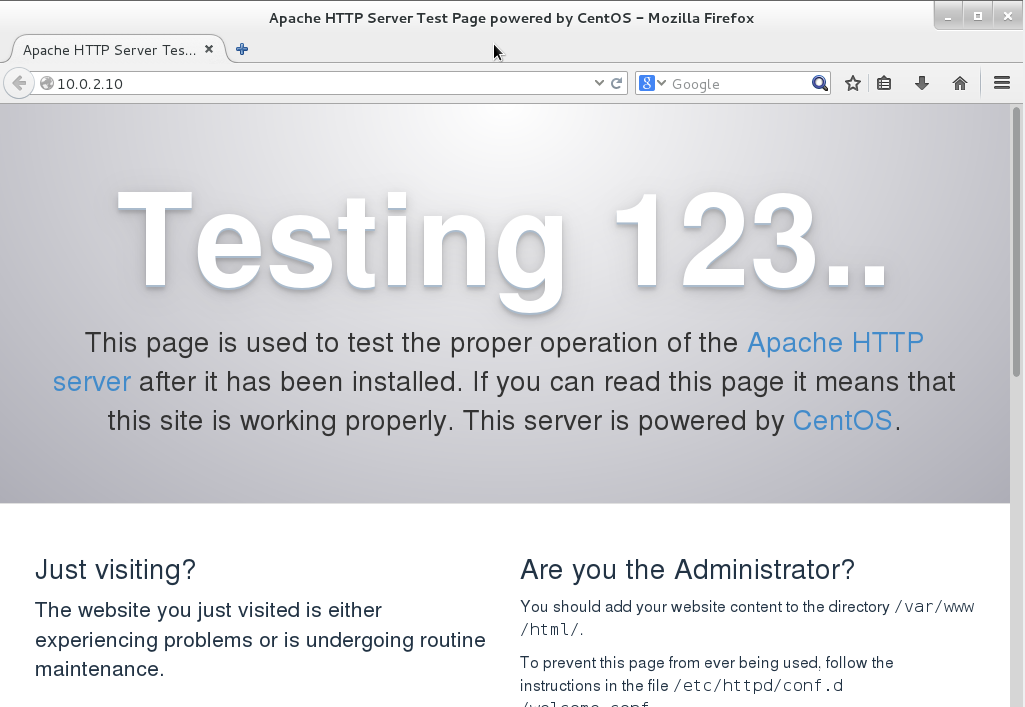
\includegraphics[width=0.75\textwidth]{18}
        \caption{Página de prueba de nuestro servidor apache}
        \label{apacheok}
    \end{figure}

    \item Una vez listo Apache, pasamos a instalar MySQL, que en este caso ser MariaDB pues MySQL no se encuentra en los repositorios de CentOS 7. Para ello ejecutamos el siguiente comando:
    \begin{minted}[frame=single, label={Instalando el servidor de base de datos}]{bash}
    sudo yum install mariadb-server mariadb
    \end{minted}

    \item Una vez instalado pasamos a activar el servicio con el siguiente comando
    \begin{minted}[frame=single, label={Arrancando el servicio de base de datos}]{bash}
    sudo service mariadb start
    \end{minted}

    \item Para establecer una contraseña root (entre otras cosas) para la base de datos lo hacemos como si de un servidor MySQL se tratase (\cite{mariadb}).
    \begin{minted}[frame=single, label={Configurando manualmente la base de datos}]{bash}
    mysql_secure_installation
    \end{minted}

    Así, tendremos que seguir los mismos pasos que seguimos en Ubuntu Server al instalar MySQL.

    \item Después de dejar listo el servidor de base de datos, pasamos a instalar PHP. Para ello, ejecutamos el siguiente comando:
    \begin{minted}[frame=single, label={Instalando PHP}]{bash}
    sudo yum install php php-mysql        
    \end{minted}

    \item En \cite{digocean2} se explica cómo buscar (\hyperref[modulosphp]{Figura \ref*{modulosphp}}), instalar y consultar (\hyperref[infomod]{Figura \ref*{infomod}}) módulos de PHP en yum para instalar en nuestro servidor:
    \begin{minted}[frame=single, label={Buscando módulos de PHP}]{bash}
    yum search php-
    \end{minted}

    \begin{figure}[!h]
        \centering
        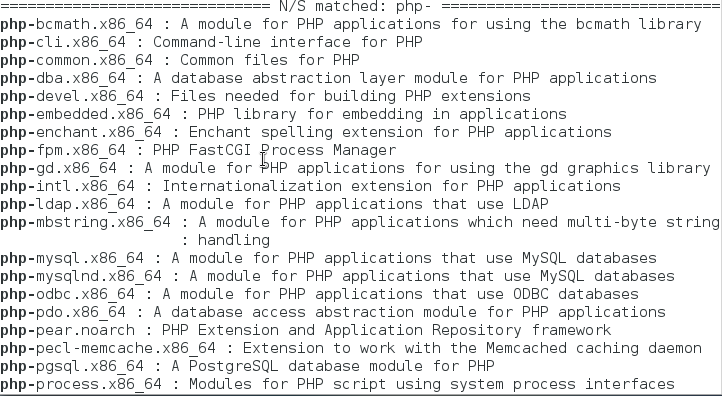
\includegraphics[width=0.5\textwidth]{19}
        \caption{Parte del output obtenido al buscar módulos de PHP}
        \label{modulosphp}
    \end{figure}

    \begin{minted}[frame=single, label={Consultando información de un módulo concreto}]{bash}
    yum info nombre_del_modulo
    \end{minted}

    \begin{figure}[!h]
        \centering
        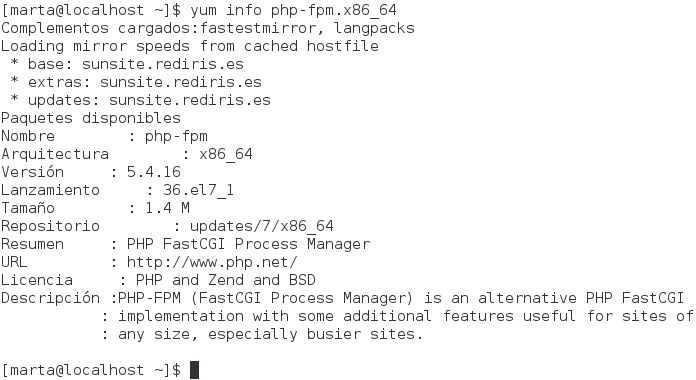
\includegraphics[width=0.5\textwidth]{20}
        \caption{Parte del output obtenido al consultar un módulo de PHP}
        \label{infomod}
    \end{figure}

    \item Por último, hacemos que al iniciar nuestro servidor, se inicie automáticamente el servidor LAMP (PHP se inicia automáticamente junto a Apache):
    \begin{minted}[frame=single, label={Automatizando el inicio de Apache y PHP al arrancar el sistema}]{bash}
    sudo chkconfig httpd on
    \end{minted}
    \begin{minted}[frame=single, label={Automatizando el inicio de MariaDB al arrancar el sistema}]{bash}
    sudo chkconfig mariadb on
    \end{minted}
\end{enumerate}

\section{Enumere otros servidores web y las páginas de sus proyectos (mínimo 3 sin considerar Apache, IIS ni nginx)}
\subsection{IBM HTTP Server}
En \cite{ibmserver} se describe este servidor web. Se incluye en un pack junto a otros productos de IBM tales como \textit{IBM WebSphere\textregistered Application Server}. Se basa en el servidor HTTP de Apache y proporciona características tales como:
\begin{enumerate}[$\bigstar$]
    \item El servidor puede administrarse remotamente
    \item Soporte para asegurar transacciones HTTPS
    \item Puede autenticar peticiones web
\end{enumerate}

\subsection{Jetty}
En \cite{jettyserver} se describe este servidor web. Es un servidor web que soporta HTTP/2, WebSocket, OSGi, JMX, JNDI, JAAS, etc. Actualmente se recomienda usar la versión 9 que es la última pero también están disponibles para descargar la versión 7 y la 8.

El proyecto está alojado en la Eclipse Foundation y algunas de sus características son:
\begin{enumerate}[$\bigstar$]
    \item Viene muy equipado y está hecho basándose en los estándares
    \item Es de código abierto y se puede usar comercialmente
    \item Es muy flexible y extendible
    \item Es escalable
\end{enumerate}

\subsection{WakandaDB}
En \cite{wakandaserver} se describe este servidor web. Es un servidor con un gestor de base de datos de código abierto con un servidor HTTP que proporciona una interfaz REST completa. 

Tanto el esquema de la base de datos, como el procesamiento del lado del servidor y el procesamiento de peticiones está todo hecho en JavaScript.

El servidor incluye las siguientes características (entre otras):
\begin{enumerate}[$\bigstar$]
    \item Conexión segura (Soporte SSL)
    \item Soporte para IPV6
    \item Conexión \textit{Keep-alive}
    \item Compresión de texto
    \item Logs del acceso a la base de datos
    \item Logs de la actividad web
\end{enumerate}

\section{Compruebe que el servicio IIS instalado está funcionando accediendo a la máquina virtual a través de la anfitriona.}
En primer lugar, comprobamos en la máquina virtual que el servidor IIS está instalado. Para ello, accedemos a internet explorer y escribimos \texttt{http://localhost} en la barra de dirección. Debemos obtener el resultado que se en la \hyperref[iisok]{Figura \ref*{iisok}}

\begin{figure}
    \centering
    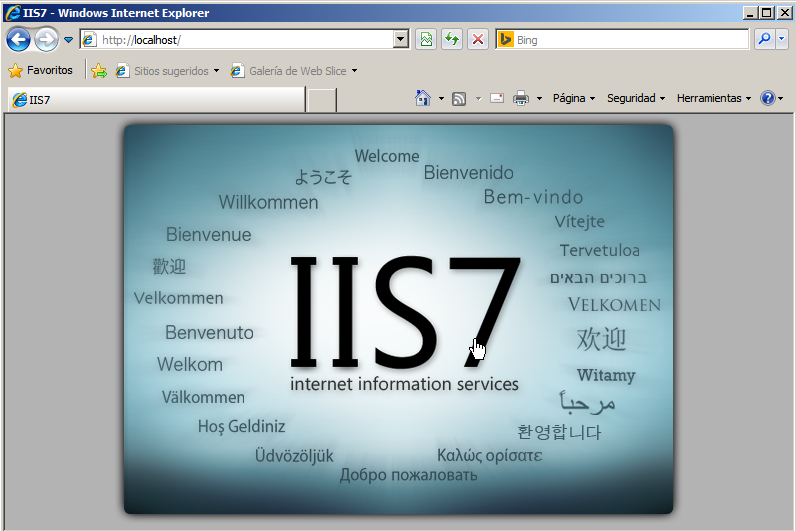
\includegraphics[width=0.7\textwidth]{21}
    \caption{Comprobación de que el servidor IIS está activo}
    \label{iisok}
\end{figure}

Tras esto, pasamos a configurar una red \textit{Host-only} en la máquina virtual para poder comunicarla con la anfitriona. Para ello seguimos los siguientes pasos:
\begin{enumerate}[1.]
    \item En Virtual Box nos vamos a \textbf{Archivo $>$ Preferencias...}. Una vez ahí seleccionamos \textbf{Red} en el menú de la izquierda y dentro de Red, seleccionamos la pestaña \textbf{Redes sólo-anfitrión}. Después, pulsamos el botón de la derecha para agregar una red sólo anfitrión. Al finalizar este paso tendremos que tenerlo todo como se ve en la \hyperref[paso1]{Figura \ref*{paso1}}.

    \begin{figure}[!h]
        \centering
        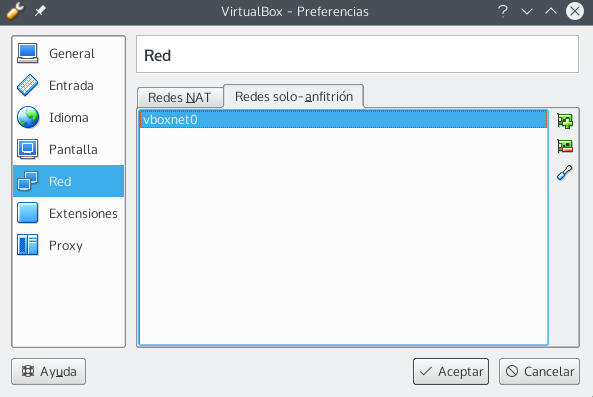
\includegraphics[width=0.7\textwidth]{23}
        \caption{Añadiendo una red sólo-anfitrión a Virtual Box}
        \label{paso1}
    \end{figure}

    Si por algún casual nos encontramos con un error a la hora de crear la red sólo-anfitrión, será necesario cerrar Virtual Box y recargar unos módulos necesarios con el comando:
    \begin{minted}[frame=single, label={Cargando los módulos que faltan en Virtual Box}]{bash}
    sudo vboxreload
    \end{minted}

    \item Una vez hemos agregado la red, pasamos a añadir una interfaz de red sólo-anfitrión a la máquina virtual. Para ello, nos vamos a la configuración de red de la máquina virtual y añadimos una red sólo-anfitrión. Al finalizar debería quedar todo como se ve en la \hyperref[paso2]{Figura \ref*{paso2}}.

    \begin{figure}[!h]
        \centering
        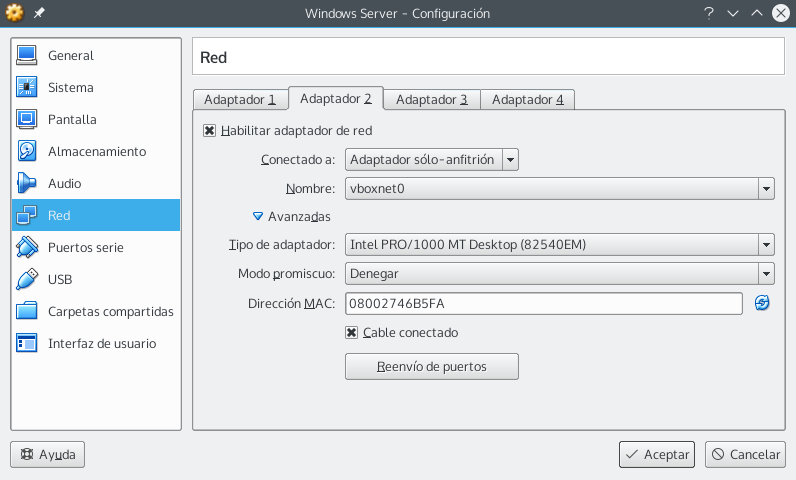
\includegraphics[width=0.7\textwidth]{24}
        \caption{Añadiendo una interfaz de red sólo-anfitrión a la máquina virtual}
        \label{paso2}
    \end{figure}

    \item En la máquina anfitriona, al hacer \texttt{ip addr} vemos que detecta la red, pero que no le ha asignado ninguna IP (\hyperref[ipaddr]{Figura \ref*{ipaddr}}), por tanto debemos asignarla nosotros de manera automática.
    \begin{figure}[!h]
        \centering
        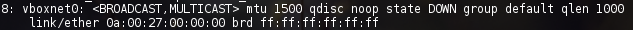
\includegraphics[width=0.7\textwidth]{25}
        \caption{Salida del comando \texttt{ip addr}, como se ve la red no tiene asignada ninguna IP}
        \label{ipaddr}
    \end{figure}

    Para asignarle una IP ejecutamos el siguiente comando
    \begin{minted}[frame=single, label={Asignando una IP a la red sólo-anfitrión}]{bash}
    sudo ip address add 192.168.56.1 dev vboxnet0
    \end{minted}

    Tras esto, al hacer \texttt{ip addr} vemos que ya sí tiene la IP que le hemos asignado (\hyperref[ipaddr2]{Figura \ref*{ipaddr2}})
    \begin{figure}[!h]
        \centering
        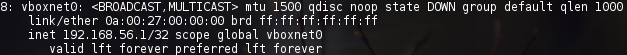
\includegraphics[width=0.7\textwidth]{26}
        \caption{Salida del comando \texttt{ip addr} tras asignarle a la red una IP}
        \label{ipaddr2}
    \end{figure}

    \item Ahora en Windows, abrimos la consola (\texttt{cmd}) y escribimos \texttt{ipconfig}. Nos fijamos en la IP de nuestro adaptador de red (\hyperref[cmd]{Figura \ref*{cmd}})
    \begin{figure}
        \centering
        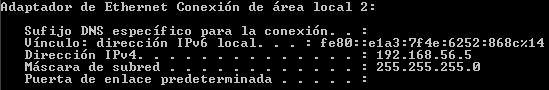
\includegraphics[width=0.7\textwidth]{27} 
        \caption{Salida que nos muestra \texttt{ipconfig} sobre el adaptador de red sólo-anfitrión}
        \label{cmd}
    \end{figure}

    \item Por último, escribimos en el navegador de la máquina anfitriona la dirección IP de la máquina virtual y debemos obtener la misma imagen que cuando lo escribimos en Internet Explorer (\hyperref[yay]{Figura \ref*{yay}}).
    \begin{figure}
        \centering
        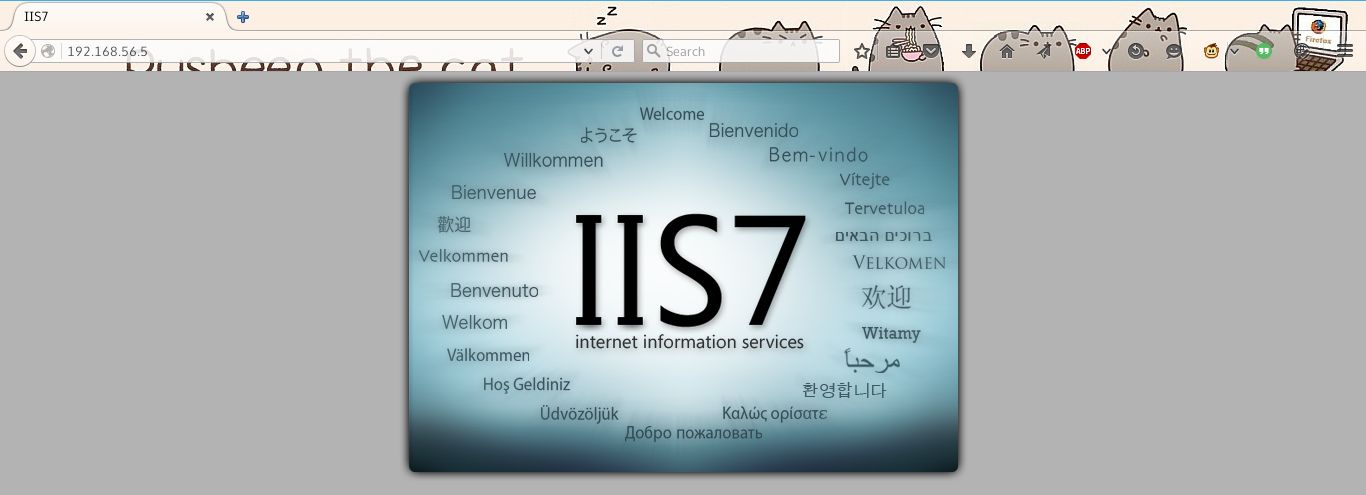
\includegraphics[width=0.7\textwidth]{22}
        \caption{Comprobación de que podemos acceder al servidor IIS instalado a través de la máquina anfitriona}
        \label{yay}
    \end{figure}
\end{enumerate}

\section{Muestre un ejemplo de uso del comando \texttt{patch}}
\label{parchefedora}
Como se ve en \cite{patchfed}, VMWare nos devuleve un error al construir el módulo \textit{vmnet}. Para solucionar ese error de forma ``rápida'' mientras se hace una actualización que lo solucione se aplica el siguiente parche:


\begin{minted}[frame=single, label={Parche para solucionar el error de VMWare}]{console}
$ curl http://pastie.org/pastes/8672356/download -o /tmp/vmware-netfilter.patch
$ cd /usr/lib/vmware/modules/source
# tar -xvf vmnet.tar
# patch -p0 -i /tmp/vmware-netfilter.patch
# tar -cf vmnet.tar vmnet-only
# rm -r vmnet-only
# vmware-modconfig --console --install-all    
\end{minted}

\subsection{Probando nuestro propio parche}
Vamos a hacer un ejemplo de uso propio siguiendo los pasos indicados en \cite{examplepatch}. Tenemos el siguiente programa:

\mycpp[label={parche.cpp}]{parche.cpp}

Como se ve, hemos cometido una falta de ortografía muy grave y vamos a corregirla con un parche. Para ello, en primer lugar corregimos el código: 

\mycpp[label={parche2.cpp}]{parche2.cpp}

Tras esto, usamos el output del comando \texttt{diff} para crear nuestro parche:
\begin{minted}[frame=single, label={Creando nuestro propio parche a partir de los dos ficheros}]{bash}
diff parche.cpp parche2.cpp > parche.patch
\end{minted}

El contenido de nuestro fichero parche sería el siguiente:
\mydiff[label={parche.patch}]{parche.patch}

Con el parche una vez creado, ejecutamos el comando \texttt{patch}, aplicando el parche a nuestro fichero \texttt{parche.cpp}
\begin{minted}[frame=single, label={Parcheando el fichero}]{bash}
patch --verbose parche.cpp < parche.patch
\end{minted}

Así, si abrimos el fichero, veremos que tiene esa gravísima falta de ortografía ya corregida. Con esto conseguimos corregimos el fallo sin necesidad de copiar y pegar el contenido del fichero \texttt{parche2.cpp}, sino de forma más elegante, aplicando un parche. Por eso, en el ejemplo anterior sobre VMWare en Fedora (visto en la \hyperref[parchefedora]{Sección \ref*{parchefedora}}), sólo hace falta descargarse el parche para poder aplicarlo.

\section{Realice la instalación de \texttt{webmin} y pruebe a modificar algún parámetro de algún servicio. Muestre las capturas de pantalla pertinentes así como el proceso de instalación}
\subsection{Instalación}
Para realizar la instalación, seguimos los pasos indicados en \cite{webmin}:

\begin{enumerate}[1.]
    \item O bien podemos descargar el archivo RPM desde la \href{http://www.webmin.com/download.html}{página web de Webmin} o bien podemos hacerlo con el siguiente comando:
\begin{minted}[frame=single, label={Descargando Webmin desde consola}]{bash}
wget http://prdownloads.sourceforge.net/webadmin/webmin-1.770-1.noarch.rpm
\end{minted}

\item Después, instalamos las dependencias con el siguiente comando:
\begin{minted}[frame=single, label={Instalando dependencias de Webmin}]{bash}
sudo yum -y install perl perl-Net-SSLeay openssl perl-IO-Tty
\end{minted}

\item Por último, para instalar Webmin ejecutamos el siguiente comando:
\begin{minted}[frame=single, label={Instalando Webmin}]{bash}
sudo rpm -U webmin-1.770-1.noarch.rpm
\end{minted}
\end{enumerate}

Tras esto se realizará la instalación automáticamente estableciendo el usuario de adminitrador a root y como contraseña, nuestra contraseña root. Ahora podríamos acceder a la URL \texttt{http://localhost:10000/} o en caso de acceder remotamente, cambiando localhost por la dirección IP de la máquina. 

Al intentarlo, obtenemos el error que se ve en la \hyperref[errorwebmin]{Figura \ref*{errorwebmin}}. En cambio, al acceder a \texttt{https://localhost:10000/} ya sí nos sale una pantalla de login como se ve en la \hyperref[webminok]{Figura \ref*{webminok}}

\begin{figure}[!h]
    \centering
    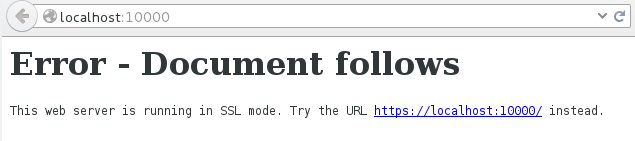
\includegraphics[width=0.7\textwidth]{28}
    \caption{Error al acceder a \texttt{http://localhost:10000/}}
    \label{errorwebmin}
\end{figure}

\begin{figure}[!h]
    \centering
    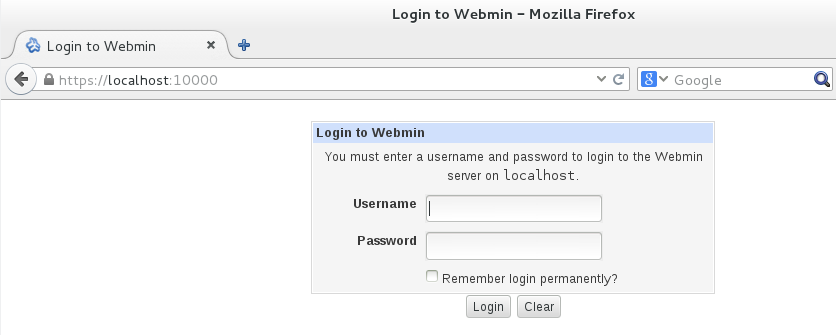
\includegraphics[width=0.7\textwidth]{29}
    \caption{Éxito al acceder a \texttt{https://localhost:10000/}}
    \label{webminok}
\end{figure}

Al loguearnos con el usuario \textit{root} y nuestra conseña root (la que usamos en el sistema) obtenemos la pantalla que se ve en la \hyperref[logwebmin]{Figura \ref*{logwebmin}} con información sobre nuestro sistema.

\begin{figure}[!h]
    \centering
    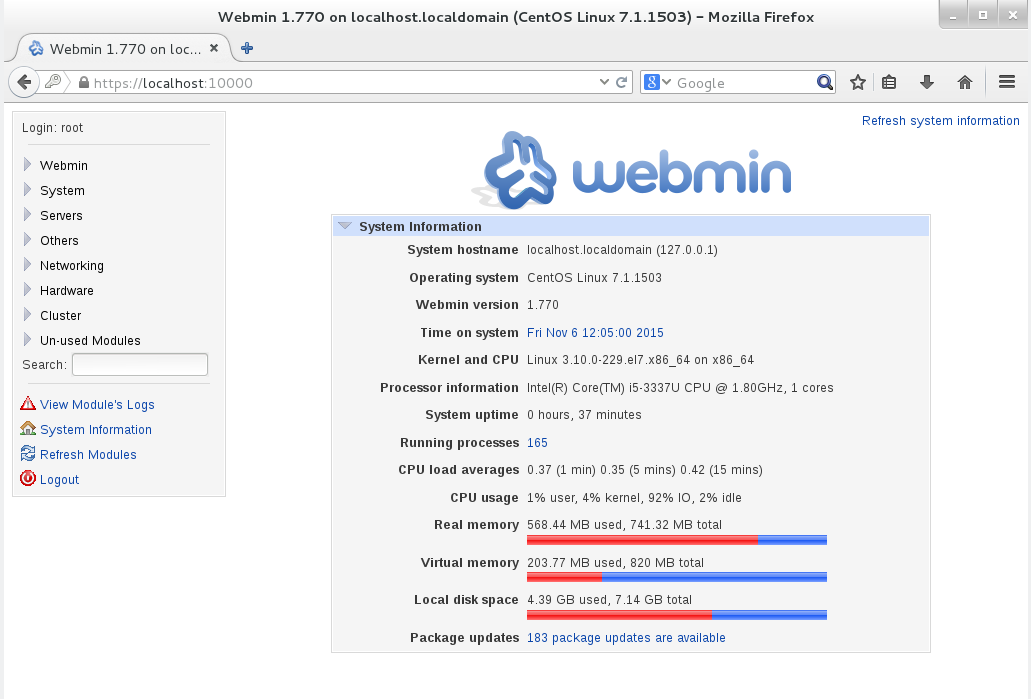
\includegraphics[width=0.7\textwidth]{30}
    \caption{Pantalla al loguearnos en webmin}
    \label{logwebmin}
\end{figure}

\subsection{Cambiando algún parámetro de Webmin}
Para ver los servicios de los que disponemos en nuestro servidor, hacemos click en \textbf{Servers} en el menú de la izquierda. Al hacer click, nos saldrán los distintos servicios que tenemos instalados y si hacemos click en uno, nos saldrán todas las operaciones que podemos hacer con dicho servicio. 

En el ejemplo de la \hyperref[sshwebmin]{Figura \ref*{sshwebmin}}, vemos que tenemos los servicios de \textit{Apache Webserver}, \textit{MySQL Database Server}, \textit{Postfix Mail Server}, \textit{Read User Mail} y \textit{SSH Server}.

\begin{figure}[!h]
    \centering
    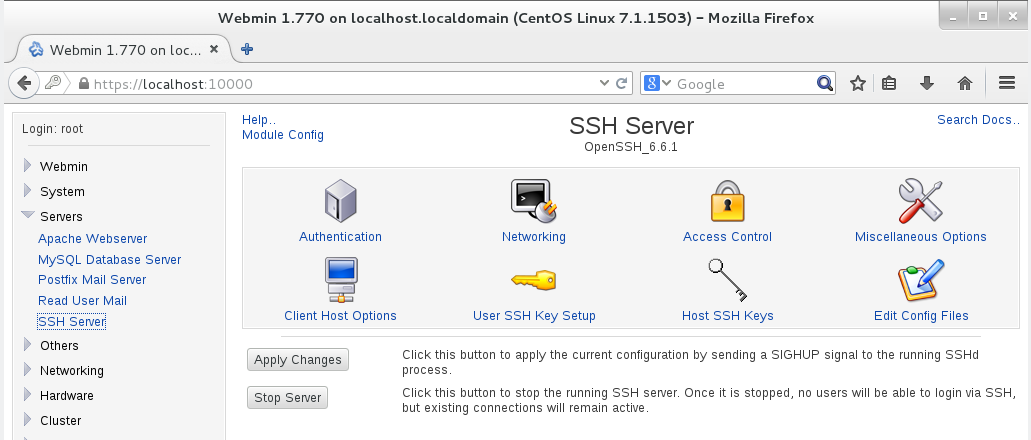
\includegraphics[width=0.7\textwidth]{31}
    \caption{Menú del servicio SSH}
    \label{sshwebmin}
\end{figure}

Si vamos a la opción de \textbf{Change config files}, nos salen los archivos de configuración del demonio ssh y de ssh. Podemos editarlos tal y como si lo estuviésemos haciendo desde consola con nano (\hyperref[sshconfigedit]{Figura \ref*{sshconfigedit}}).

\begin{figure}[!h]
    \centering
    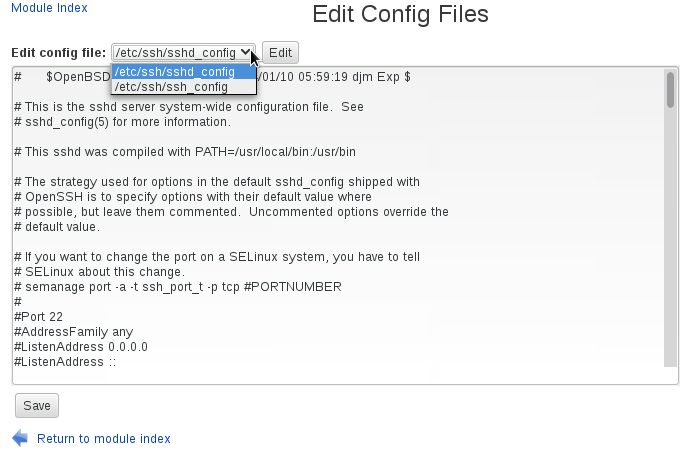
\includegraphics[width=0.7\textwidth]{32}
    \caption{Editando el archivo de configuración del demonio SSH}
    \label{sshconfigedit}
\end{figure}

En nuestro caso, vamos a NO permitir que se loguee el usuario root a través de SSH. Para ello, descomentamos la línea \texttt{\# PermitRootLogin yes} y cambiamos ese yes por un no. Tras esto, le damos al botón de \textit{Save} y volveremos al menú principal de nuestro servidor SSH. En dicho menú debemos de darle al botón de \textit{Apply Changes} para guardar los cambios que hemos hecho en el servidor SSH.

Al intentar loguearnos con el usuario root, nos dirá que no tenemos permiso para ello. Sin embargo, al loguearnos con cualquier otro usuario, lo haremos exitosamente (\hyperref[sshloginroot]{Figura \ref*{sshloginroot}}).

\begin{figure}[!h]
    \centering
    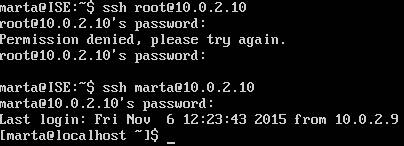
\includegraphics[width=0.7\textwidth]{33}
    \caption{No podemos loguearnos con el usuario root pero sí con otros usuarios}
    \label{sshloginroot}
\end{figure}

\section{Instale \texttt{phpMyAdmin}, indique cómo lo ha realizado y muestre algunas capturas de pantalla. Configure PHP para poder importar BDs mayores de 8MiB (límite por defecto). Indique cómo ha realizado el proceso y muestre capturas de pantalla}
Para instalar \texttt{phpMyAdmin}, utilizamos el siguiente comando:

\begin{minted}[frame=single, label={Instalando phpMyAdmin}]{bash}
sudo apt-get install phpMyAdmin
\end{minted}

Tras confirmar la instalación nos saldrá una ventana para elegir el servidor web que se configurará para que ejecute \texttt{phpMyAdmin}. Nosotros elegimos \texttt{apache2} (\hyperref[serverphpmyadmin]{Figura \ref*{serverphpmyadmin}}).

\begin{figure}[!h]
    \centering
    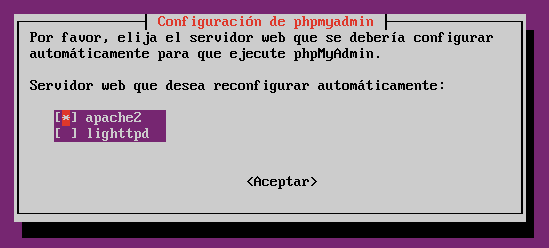
\includegraphics[width=0.7\textwidth]{34}
    \caption{Eligiendo el servidor que ejecutará \texttt{phpMyAdmin}}
    \label{serverphpmyadmin}
\end{figure}

Después, nos saldrá un mensaje diciendo si queremos que \texttt{phpMyAdmin} configure automáticamente una base de datos o si queremos hacerlo nosotros. Nosotros le decimos que sí. (\hyperref[bdphpmyadmin]{Figura \ref*{bdphpmyadmin}}). Tras esto, nos pedirá una contraseña para el administrador de la base de datos, una contraseña de aplicación MySQL para phpMyAdmin y finalizará la instalación.


Para configurar PHP, según \cite{phpini}, debemos modificar el archivo \textbf{php.ini} localizado en \textit{/etc/php5/apache2/php.ini}. En dicho fichero buscamos \textbf{post\_max\_size}, \textbf{memory\_limit} y \textbf{upload\_max\_filesize}. Incrementamos los valores de estos los dos últimos a 10000M y dejamos el de \textbf{post\_max\_size} a 0. Tras esto reiniciamos el servicio apache y como se ve en la \hyperref[postmaxsize]{Figura \ref*{postmaxsize}}, al subir la base de datos de 35MB podemos hacerlo con éxito.

\begin{figure}[!h]
    \centering
    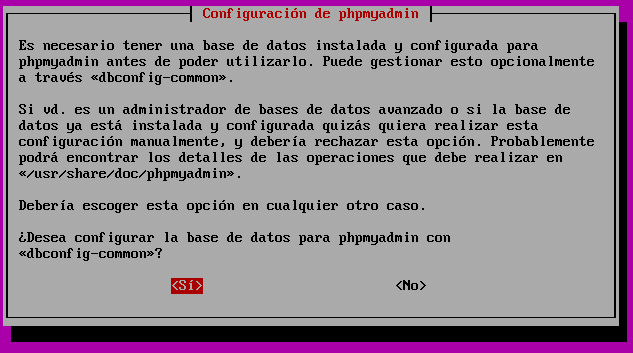
\includegraphics[width=0.7\textwidth]{35}
    \caption{Configuración de la base de datos de \texttt{phpMyAdmin}}
    \label{bdphpmyadmin}
\end{figure}

\begin{figure}[!h]
    \centering
    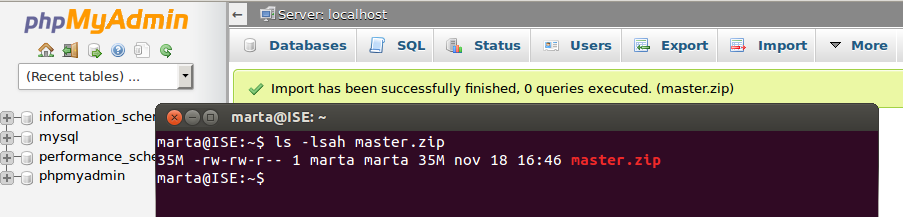
\includegraphics[width=0.7\textwidth]{36}
    \caption{Tras cambiar los parámetros indicados, hemos podido importar una base de datos de 35MB}
    \label{postmaxsize}
\end{figure}

Para comprobar que funciona, he descargado la base de datos disponible en \cite{testdb} y la he importado a mi base de datos a través de \texttt{http://localhost/phpmyadmin}.

\section{Visite la web de \textit{ISPConfig} y pruebe la demo que ofrecen realizando capturas de pantalla y comentando qué está realizando.}

Si entramos en la web de ISPConfig y hacemos click en \href{http://www.ISPConfig.org/page/en/ISPConfig/online-demo.html}{Online Demo}, accederemos al panel de control online. Tenemos tres opciones para acceder:
\begin{enumerate}[$\bullet$]
    \item Acceder como \textbf{administrador}, para lo cual tenemos que loguearnos con el nombre de usuario \textbf{admin} y la contraseña \textbf{demo}. Al hacer esto obtenemos la pantalla de la \hyperref[admin]{Figura \ref*{admin}}.

    \begin{figure}[!h]
        \centering
        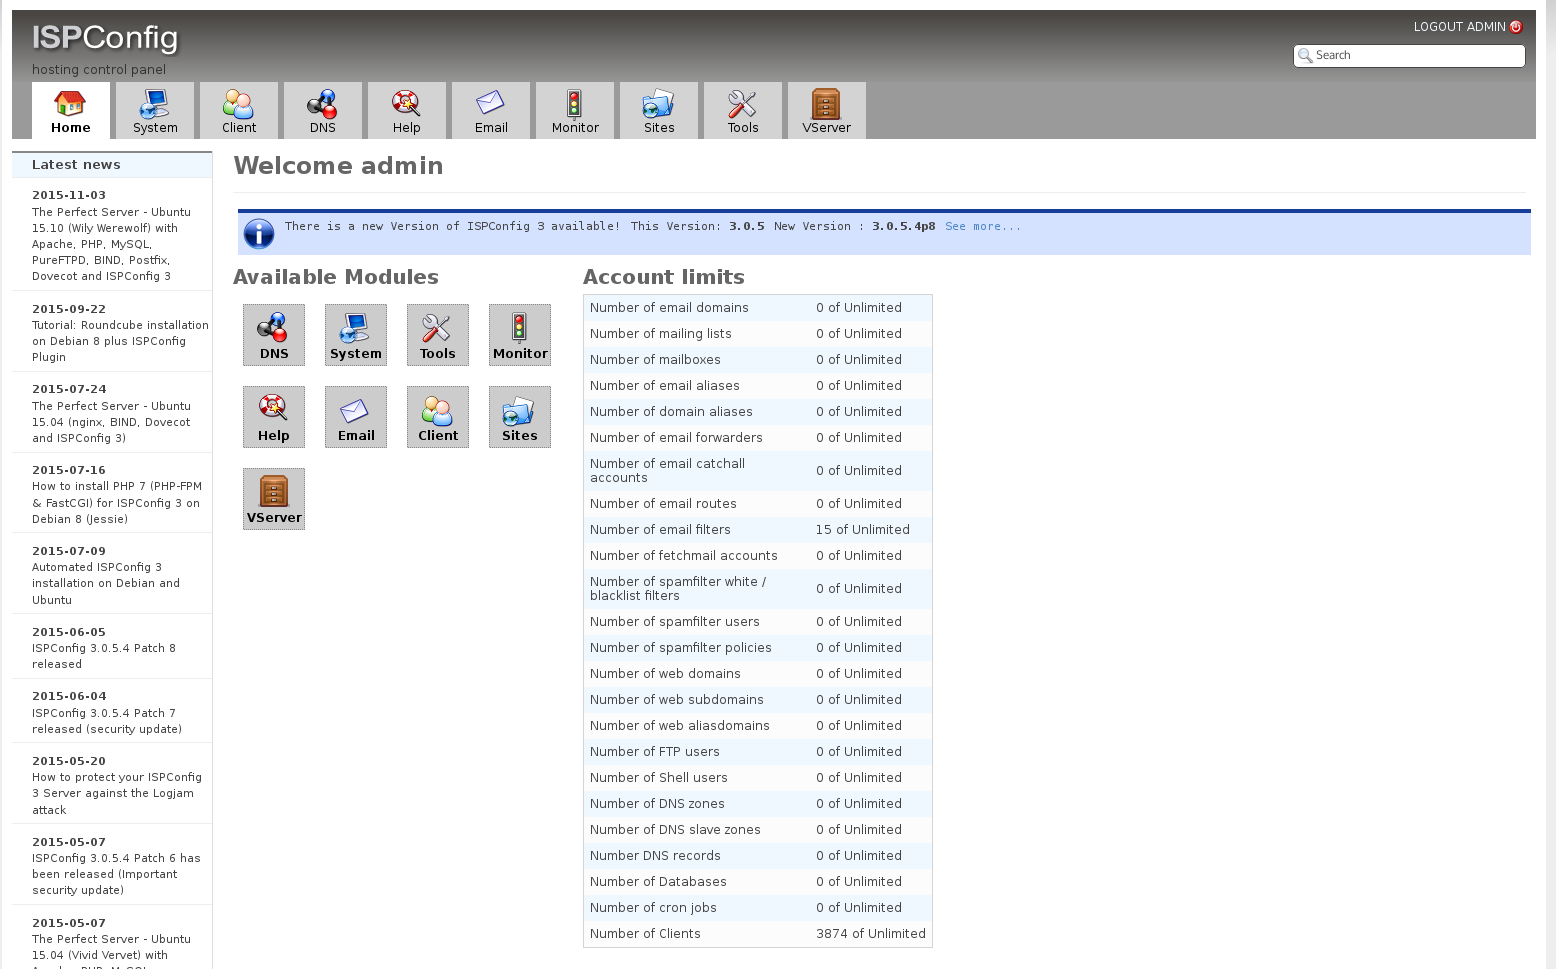
\includegraphics[width=0.5\textwidth]{37}
        \caption{Pantalla al acceder a ISPConfig como administrador}
        \label{admin}
    \end{figure}

    \item Acceder como \textbf{cliente}, para lo cual tenemos que loguearnos con el nombre de usuario \textbf{client} y la misma contraseña. Al hacer esto, obtenemos una interfaz con una funcionalidad más limitada respecto a la de administrador (\hyperref[client]{Figura \ref*{client}}).

    \begin{figure}[!h]
        \centering
        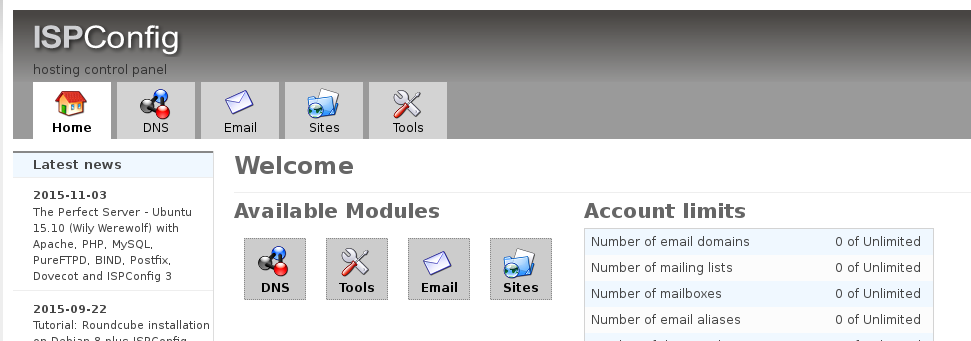
\includegraphics[width=0.5\textwidth]{38}
        \caption{Pantalla al acceder a ISPConfig como cliente}
        \label{client}
    \end{figure}

    \item Acceder como \textbf{\textit{reseller}}, para lo cual tenemos que loguearnos con el nombre de usuario \textbf{reseller} y la misma contraseña. Al hacer esto, obtenemos una interfaz con un poco más de funcionalidad que la de cliente (\hyperref[reseller]{Figura \ref*{reseller}}).

    \begin{figure}[!h]
        \centering
        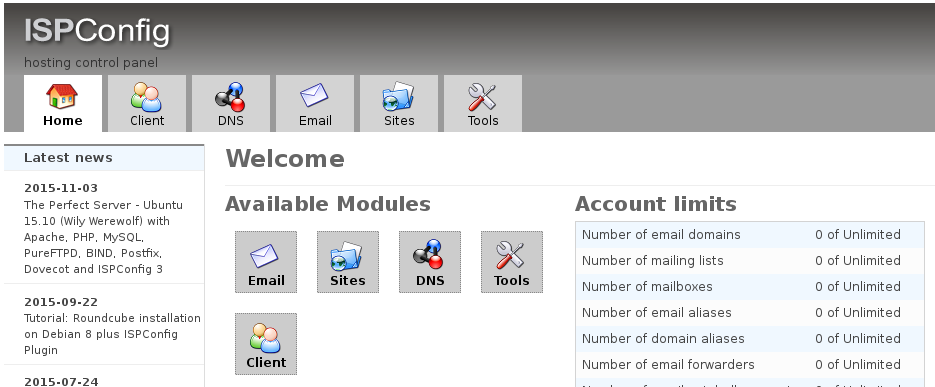
\includegraphics[width=0.5\textwidth]{39}
        \caption{Pantalla al acceder a ISPConfig como \textit{reseller}}
        \label{reseller}
    \end{figure}
\end{enumerate}

Una función muy interesante de ISPConfig es la de \textbf{Monitorizar el sistema}. Nos permite ver el estado del RAID, la carga del servidor, el uso de memoria y archivos de logs varios.

También podemos configurar aspectos del servidor tales como \textbf{añadir una nueva dirección IP} (y mostrar las actuales) (\hyperref[ipdir]{Figura \ref*{ipdir}}) o configurar el lugar desde el que nos descargamos actualizaciones.

\begin{figure}[!h]
\centering
\mbox {
\subfigure[Mostrando las direcciones IP del sistema]{
\label{showips}
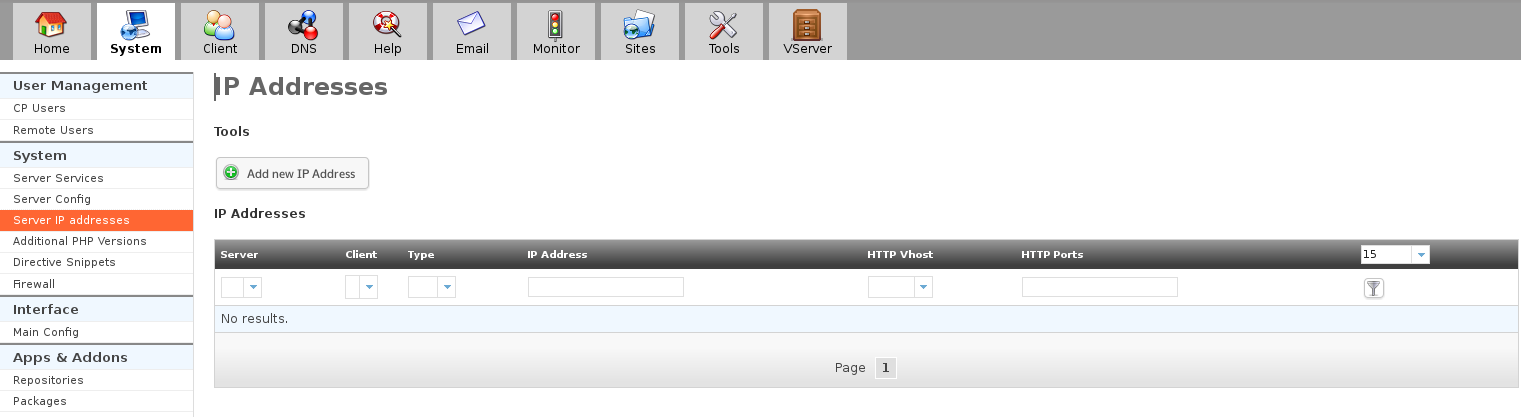
\includegraphics[width=0.5\textwidth]{40}
}
\qquad
\subfigure[Añadiendo una nueva dirección IP] {
\label{addips}
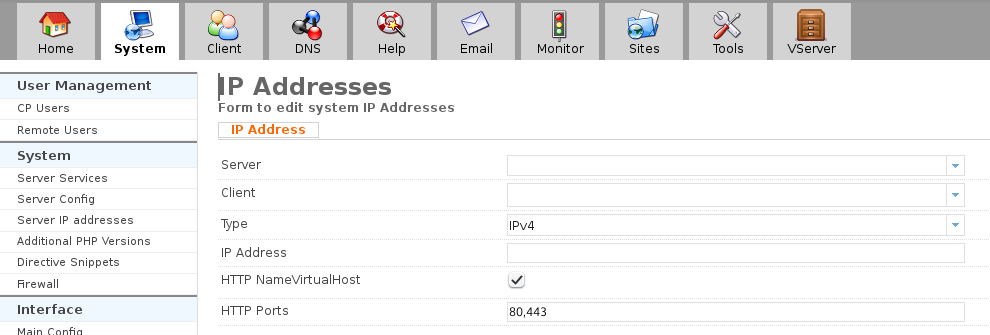
\includegraphics[width=0.5\textwidth]{41}
}
}
\caption{Direcciones IP}
\label{ipdir}
\end{figure}

\section{Ejecute los ejemplos de \texttt{find}, \texttt{grep} y escriba el script que haga uso de \texttt{sed} para cambiar la configuración de ssh y reiniciar el serivicio}
\subsection{\texttt{grep}}
Al ejecutar \texttt{ps -Af} obtenemos una lista enorme, en la \hyperref[psaf]{Figura \ref*{psaf}} sólo se ve una pequeña parte. Si queremos buscar un proceso determinado en la lista podemos pasar un buen rato buscando. Aquí viene la utilidad del comando \texttt{grep}, y es que si sabemos el nombre del proceso determinado que buscamos \texttt{grep} lo filtrará por nosotros ahorrándonos la tarea. En el ejemplo de la \hyperref[psafyaku]{Figura \ref*{psafyaku}}, se ha querido buscar el proceso \textit{yakuake} en la lista de procesos en ejecución.

\begin{figure}[!h]
    \centering
    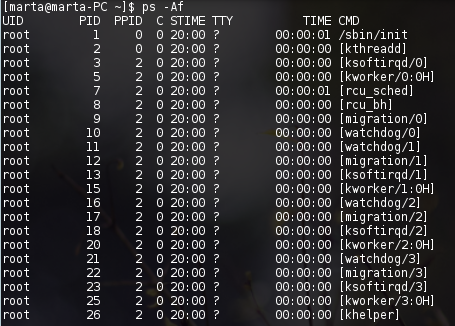
\includegraphics[width=0.7\textwidth]{42}
    \caption{Parte del output de \texttt{ps -Af}}
    \label{psaf}
\end{figure}

\begin{figure}[!h]
    \centering
    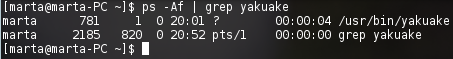
\includegraphics[width=0.7\textwidth]{43}
    \caption{Parte del output de \texttt{ps -Af | grep yakuake}}
    \label{psafyaku}
\end{figure}

\subsection{\texttt{find}}
Si queremos buscar todos los archivos PDF que tenemos en nuestra carpeta de Descargas y copiarlos todos a otra carpeta, podemos o bien ir con nuestro gestor de archivos gráfico (como por ejemplo \textit{Dolphin}) carpeta a carpeta buscando cada archivo PDF y copiándolo a nuestra carpeta, o bien podemos hacer lo mismo pero por consola (jugando con los comandos \texttt{cd}, \texttt{ls} y \texttt{cp}) o bien podemos usar el comando \texttt{find}.

Con \texttt{find} podemos buscar todos los archivos cuyo nombre coincidan con una expresión regular dada (en nuestro ejemplo, los archivos cuyo nombre coincida con la expresión regular $*.pdf$) y aplicar una acción sobre ellos:

\begin{minted}{bash}
find /home/marta/Descargas -name '*.pdf' -exec cp {} ~/PDFs \;
\end{minted}

Para que el comando funcione, debe haber previamente una carpeta en nuestro home que se llame PDFs ya que si no, \texttt{find} nos creará un archivo en nuestra carpeta home llamado \textit{PDFs} en vez de un directorio. Una vez hecho, si hacemos un \texttt{ls} vemos que todos los PDFs que había en la carpeta de Descargas están ahora también en la carpeta PDFs.

\subsection{\texttt{sed}}
Según \cite{mansed}, el comando en \texttt{sed} para realizar sustituciones es \texttt{s/regexp/replacement/} donde \texttt{regexp} es la expresión que va a buscar en el fichero para sustituir y \texttt{replacement} la expresión por la que será sustituida.


Así, en nuestro caso le daremos llamaríamos al programa con algo así como \texttt{sed 's/PermitRootLogin yes/PermitRootLogin no/' < sshd\_config > sshd\_config1}. Ya que si lo ejecutamos sobre el mismo fichero (\texttt{< sshd\_config > sshd\_config}) se perdería el contenido. 

Por tanto, nuestro script también debería tener, tras la ejecución de \texttt{sed}, otro comando para copiar el contenido de un fichero a otro y borrar el ``auxiliar'' creado.

\mybash[label={sed.sh}]{sed.sh}

En la \hyperref[ejemploej]{Figura \ref*{ejemploej}}, se ve un ejemplo de ejecución del script.

\begin{figure}[!h]
\centering
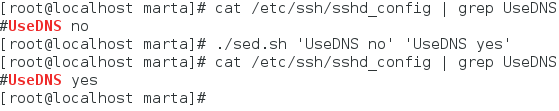
\includegraphics[width=0.7\textwidth]{44}
\caption{Ejemplo de ejecución del script}
\label{ejemploej}
\end{figure}

\section{Escriba el script para cambiar el acceso a ssh usando Python}
Para hacer el script, necesitamos lo siguiente:
\begin{enumerate}[---]
    \item Alguna forma de poder modificar el contenido de un archivo
    \item Alguna forma de detectar cuando se ha modificado dicho archivo para reiniciar el demonio SSH
\end{enumerate}

Para modificar el archivo se ha usado el módulo descrito en \cite{docreplace} y para reiniciar el servicio SSH, haré un \textit{Playbook} tal y como se describe en \cite{handler}.

\subsection{Servidores conocidos}
En primer lugar, debemos hacer un archivo con servidores conocidos a los que nos conectaremos. Dicho archivo es \textit{/etc/ansible/hosts} y tiene la estructura que se ve en la \hyperref[hostansi]{Figura \ref*{hostansi}}.

\begin{figure}[!h]
    \centering
    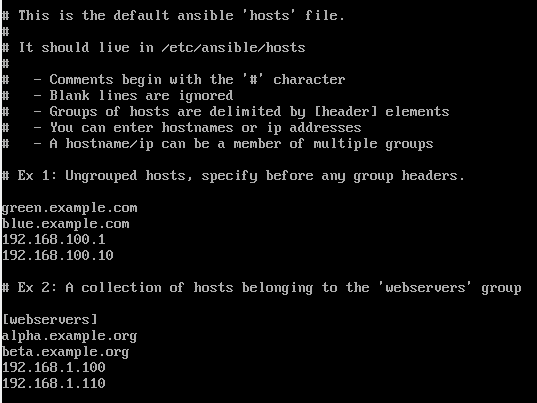
\includegraphics[width=0.7\textwidth]{45}
    \caption{Fichero de host por defecto de Ansible}
    \label{hostansi}
\end{figure}

En mi caso, sólo he añadido la máquina virtual de CentOS. Para comprobar que se ha añadido de forma correcta, hacemos un \texttt{ping} a todos nuestros host a través de ansible y debemos obtener un mensaje como el de la \hyperref[pingpong]{Figura \ref*{pingpong}}.

\begin{figure}[!h]
    \centering
    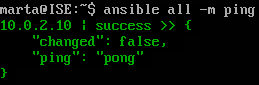
\includegraphics[width=0.5\textwidth]{46}
    \caption{Haciendo \texttt{ping} a todos los host guardados}
    \label{pingpong}
\end{figure}

\subsection{Haciendo el \textit{Playbook}}
Siguiendo las indicaciones de \cite{playbook}, he hecho el siguiente \textit{Playbook}:

\myyml[label={ssh.yml}]{ssh.yml}

Para ejecutarlo, debemos hacerlo con el siguiente comando:
\begin{minted}[frame=single, label={Ejecutando el script de Ansible}]{bash}
ansible-playbook -k ssh.yml --extra-vars='exp="exp a buscar" rep="exp a reemplazar"'
\end{minted}

Así por ejemplo, para cambiar el parámetro \texttt{UseDNS} de yes a no lo haríamos como se ve en la \hyperref[ansible]{Figura \ref*{ansible}}.

\begin{figure}[!h]
    \centering
    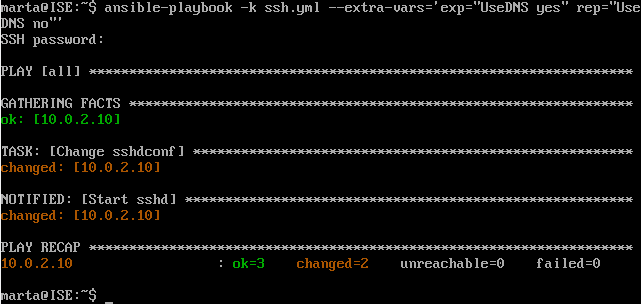
\includegraphics[width=0.7\textwidth]{47}
    \caption{Script para cambiar un parámetro de SSH}
    \label{ansible}
\end{figure}

\section{Abra una consola de Powershell y pruebe a parar un programa en ejecución (p.ej), realice capturas de pantalla y comente lo que muestra}
Vamos a probar a parar la ejecución de \textit{Internet Explorer}, para ello, comprobamos en primer lugar que se está ejecutando con el comando

\begin{minted}[frame=single, label={Comprobando que estamos ejecutando Internet Explorer}]{powershell}
Get-Process -Name iexplore
\end{minted}

Tras esto, lo detenemos con el comando
\begin{minted}[frame=single, label={Deteniendo Internet Explorer}]{powershell}
Stop-Process -Name iexplore
\end{minted}

Al volver a ejecutar el comando \texttt{Get-Process} obtenemos un error. En la \hyperref[ie]{Figura \ref*{ie}} se ve este proceso.

\begin{figure}[!h]
    \centering
    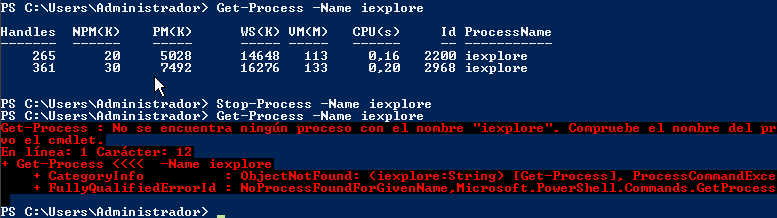
\includegraphics[width=0.7\textwidth]{48}
    \caption{Deteniendo la ejecución de Internet Explorer}
    \label{ie}
\end{figure}  

\section{Cuestiones Opcionales}
\subsection{¿Qué gestores utiliza OpenSuse?}
En la sección \textit{Gestor de paquetes} de \cite{wikisuse} se explica que hay dos gestores de paquetes en openSUSE:
\begin{enumerate}[$\bullet$]
    \item \textbf{YaST}: es un gestor de paquetes con interfaz gráfica.
    \item \textbf{Zypper}: es un gestor de paquetes desde la línea de comandos. En \cite{zypper} podemos encontrar una guía de uso de este gestor de paquetes.
\end{enumerate}

\subsection{Instale y pruebe terminator. Con screen, pruebe su funcionamiento dejando sesiones ssh abiertas en el servidor y recuperándolas posteriormente}
Mi experiencia con terminator se resume en la \hyperref[terminator]{Figura \ref*{terminator}}. He probado a partir la pantalla, poner un perfil distinto en cada división y, trabajar en tareas independientes en cada terminal de forma paralela.

\begin{figure}[!h]
\centering
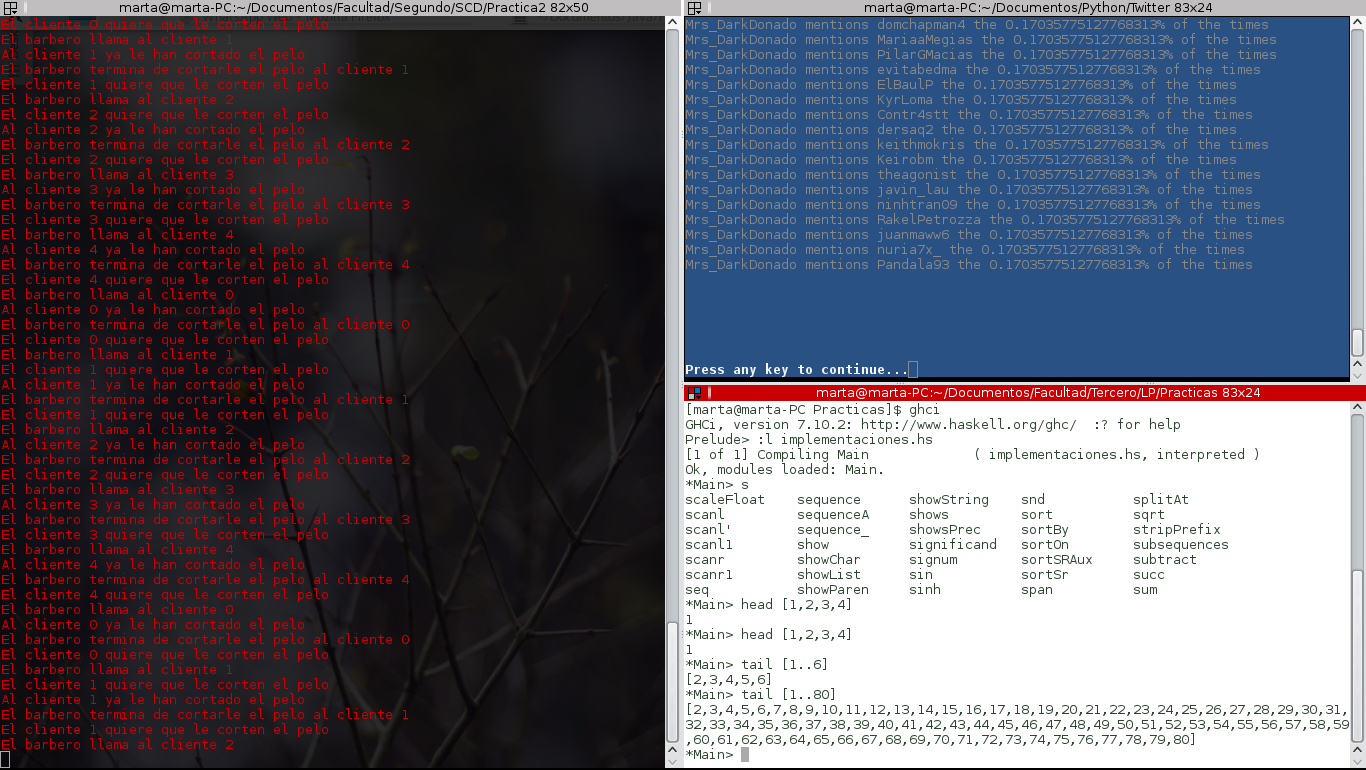
\includegraphics[width=0.75\textwidth]{16}
\caption{Prueba con terminator}
\label{terminator}
\end{figure}

En \cite{screen}, se explica un funcionamiento básico de screen. En nuestro caso, tendremos dos sesiones de screen abiertas.

Probamos a abrir una sesión ssh en la sesión 1, y pulsando \textbf{Control+a+d} la suspendemos. Tras esto, se cierra la sesión, pero podemos listar las sesiones de screen actualmente en funcionamiento con el comando:

\begin{minted}[frame=single, label={listando las sesiones de screen actuales}]{bash}
screen -ls
\end{minted}

\begin{figure}[!h]
\centering
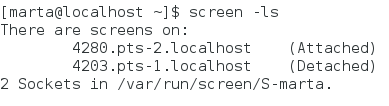
\includegraphics[width=0.75\textwidth]{51}
\caption{Listando las sesiones de \texttt{screen} actualmente abiertas}
\label{screenlist}
\end{figure}

Como se ve en la \hyperref[screenlist]{Figura \ref*{screenlist}} tenemos una sesión suspendida. Para recuperarla usamos la opción \texttt{-r} acompañada del ID de dicha sesión:

\begin{minted}[frame=single, label={Reanudando la sesión ssh que teníamos en screen}]{bash}
screen -r 4203 
\end{minted}

También probamos el modo de \textit{split window}. Para ello, pulsamos \textbf{Control+a+S}, tras esto, nos movemos a la nueva ventana que hemos hecho con \textbf{Control+a+Tab} y una vez ahí pulsamos \textbf{Control+a+c} para empezar una nueva sesión de screen. El resultado es el que se ve en la \hyperref[split]{Figura \ref*{split}}. 

\begin{figure}[!h]
\centering
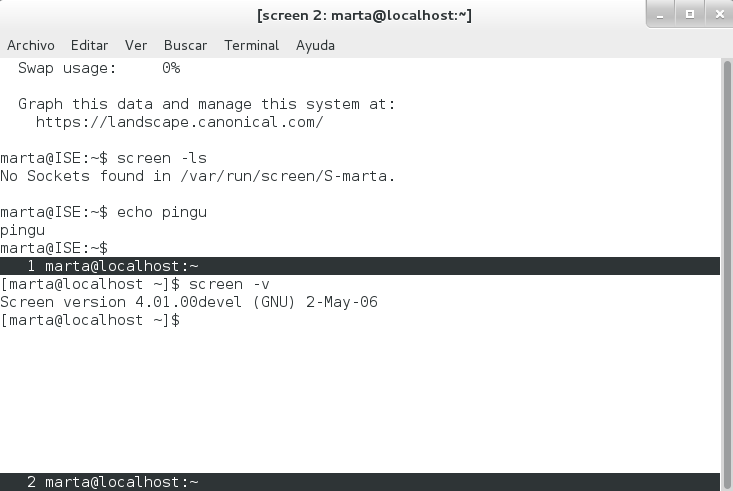
\includegraphics[width=0.75\textwidth]{17}
\caption{Haciendo un split en la sesión de screen actual}
\label{split}
\end{figure}

\subsection{Instale el servicio \texttt{fail2ban} y pruebe su funcionamiento}
Para instalar \texttt{fail2ban} en Ubuntu Server ejecutamos el comando bien conocido:
\begin{minted}[frame=single, label={Instalación de fail2ban en Ubuntu Server}]{bash}
sudo apt-get install fail2ban    
\end{minted}

Una vez hecho esto, consultamos \cite{fail2banwiki} para saber cómo se usa y cómo se configura. En primer lugar tenemos un cliente y un servidor:
\begin{enumerate}[---]
    \item \texttt{fail2ban-client}: es el \textit{frontend} de Fail2ban. Se conecta al servidor definido en el archivo socket y le envía comandos para configurar y operar el servidor. El cliente puede leer archivos de configuración o usarse para mandar órdenes al servidor. Sus opciones son:
    \begin{enumerate}[$\bullet$]
        \item \texttt{-c <DIR>}: directorio de configuración. Por defecto \textit{/etc/fail2ban}
        \item \texttt{-s <FILE>}: ruta del socket
        \item \texttt{-d}: configuración ``\textit{dump}'', para depurar.
        \item \texttt{-i}: modo interactivo
        \item \texttt{-v}: aumenta la cantidad de información que nos muestra el programa
        \item \texttt{-q}: disminuye la cantidad de información que nos muestra el programa
        \item \texttt{-x}: fuerza la ejecución del servidor
        \item \texttt{-h}: ayuda
        \item \texttt{-V}: muestra la versión
    \end{enumerate}
    \item \texttt{fail2ban-server}: el servidor inicialmente no tiene definida ninguna ``cárcel''. No debe usarse directamente, excepto cuando se está depurando. Dispone de las siguientes opciones:
    \begin{enumerate}[$\bullet$]
        \item \texttt{-b}: empieza el programa en segundo plano
        \item \texttt{-f}: empieza el programa en primer plano
        \item \texttt{-s <FILE>}: ruta del socket
        \item \texttt{-x}: fuerza la ejecución del servidor
        \item \texttt{-h}: muestra un mensaje de ayuda
        \item \texttt{-V}: muestra la versión
    \end{enumerate}
\end{enumerate}

Para hacer una simple prueba, iniciamos \texttt{fail2ban} con la configuración por defecto:
\begin{minted}[frame=single, label={Iniciamos fail2ban}]{bash}
sudo fail2ban-client -v start
\end{minted}

Como información nos da que el archivo socket en uso es \textit{/var/run/fail2ban/fail2ban.sock}.

Si usamos la opción \texttt{-i}, nos saldrá algo parecido a cuando usamos ftp para introducir comandos, \texttt{fail2ban>}.

Si miramos el archivo \textit{jail.conf}, podemos configurar cosas tales como las IP que no queremos banear, el tiempo que un host queda baneado, los parámetros para banear a un host (número de peticiones que genera en un tiempo determinado), etc. 

También podemos configurar los distintos servicios que queremos controlar, por ejemplo: ssh, xinetd, apache, vsftp, etc.

% \subsection{Realice la instalación de uno de estos dos ``web containers'' (\textit{Apache Tomcat} o \textit{Jboss}) y pruebe su ejecución.}

% Hemos elegido el \textit{Apache Tomcat}. Para descargarlo hemos entrado en \href{http://tomcat.apache.org/download-80.cgi}{Download Tomcat 8.0}, en el menú de la izquierda. Una vez ahí, hemos escogido la versión para Windows de 64 bits.

% Una vez descargado, abrimos el archivo \textbf{RUNNING}, en el cual se nos indica que para ejecutar el programa debemos tener instalado \href{http://www.oracle.com/technetwork/java/javase/downloads/index.html}{Java SE Runtime Environment (JRE)}.

\setcounter{subsection}{5}

% \subsection{Realice la instalación de MongoDB en alguna de sus máquinas virtuales. Cree una colección de documentos y haga una consulta sobre ellos.}
% Siguiendo los pasos indicados en \cite{installmongo}:
% \begin{enumerate}[1.]
% \item En primer lugar creamos el archivo de repositorio de MongoDB para ello ejecutamos el siguiente comando:
% \begin{minted}[frame=single, label={Creando el archivo de repositorio de MongoDB}]{bash}
% sudo touch /etc/yum.repos.d/mongodb-org-3.0.repo
% \end{minted}

% \item Le damos contenido al archivo, en concreto el contenido que se ve en la \hyperref[repo]{Figura \ref*{repo}}.

% \begin{minted}[frame=single, label={Dando contenido al archivo}]{bash}
% sudo nano /etc/yum.repos.d/mongodb-org-3.0.repo
% \end{minted}

% \begin{figure}[!h]
%     \centering
%     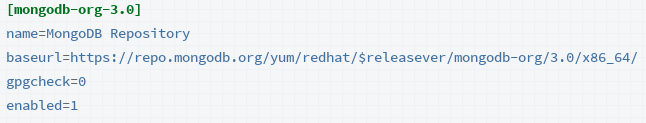
\includegraphics[width=0.7\textwidth]{50}
%     \caption{Contenido del archivo de configuración del repositorio de MongoDB}
%     \label{repo}
% \end{figure}

% \item Tras esto, instalamos MongoDB con \texttt{yum}:
% \begin{minted}[frame=single, label={Instalando MongoDB}]{bash}
% sudo yum install -y mongodb-org
% \end{minted}

% \item Una vez instalado, debemos configurar SELinux para permitir que MongoDB arranque. Para ello, establecemos el parámetro \texttt{SELINUX} del archivo \textit{/etc/selinux/config} a \texttt{permissive}.
% \begin{minted}[frame=single, label={Configurando SELinux}]{bash}
% sudo nano /etc/selinux/config
% SELINUX=permissive
% \end{minted}

% \item Reiniciamos el sistema.

% \item Iniciamos el servicio, para ello usamos el siguiente comando:
% \end{enumerate}

\subsection{Muestre un ejemplo de uso para \texttt{awk}}
En \cite{manawk} se ponen algunos ejemplos de uso de \texttt{awk}. Un ejemplo es \textit{preceder cada línea de su número en un archivo}. Esto se haría con el siguiente comando \texttt{awk}:
\begin{minted}[frame=single, label={Añadiendo a cada linea su numero de linea}]{bash}
awk -F: '{ nlines++; print nlines, $0; }' hola.txt
\end{minted}

Un ejemplo de uso se ve en la \hyperref[awkej]{Figura \ref*{awkej}}.

\begin{figure}[!h]
    \centering
    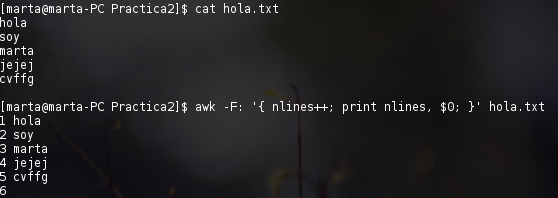
\includegraphics[width=0.7\textwidth]{49}
    \caption{Ejemplo de uso del comando \texttt{awk}}
    \label{awkej}
\end{figure}

\bibliography{P2-MarGomMac.bib} %archivo citas.bib que contiene las entradas 
\bibliographystyle{siam} % haycle varias formas de citar

\end{document}